\chapter{Segregation theory}
\label{app:segreg}

\section{Physical context}

In this appendix, I will give a simple derivation of the equation we used to model the segregation process taking place in granular flows.

We consider a granular flow going down a slope. For the sake of simplicity, we will assume that the granular material is a mixture of small and large particles. This assumption is commonly made, since it simplifies greatly the equations, but still captures the essential physical features of segregation. Through this section $s$ and $l$ superscripts will respectively refer to small and large particles. For example the mass of a small particle will be labelled $m^s$.
As usual, we model the granular flow using the tools of continuum mechanics. 

The idea is to see the set of large particles in the material as a matrix through the holes of which small particles can fall. 
If the material is a still, initially homogeneous mixture of small and large particles, it will partially segregate (leaving the uppermost layers full of large particles, the lowermost full of small particles.). In this case middle layers are a mixture of small and large particles.
If the material is a flowing, initially homogeneous mixture of small and large particles, it will completely segregate. This is because as the material flows down the slope, the local void ratio of the large particles matrix fluctuate, causing small to fall into newly opening gaps. The result is a progressive migration of small particles to the bottom. Because of force imbalance, large particles are pushed upward as small particles go downward. After some time, the material will be constituted of a layer of large particles topping a layer of small particles.

\section{Derivation of the segregation equation}

Let us start by writing down the momentum and force balances for each one of the 2 constituents

\begin{equation} \label{eq:mom_bal}
	\partial_t \rho^\nu u_i^\nu + \partial_j \rho^\nu u_i^\nu u_j^\nu = -\partial_i p^\nu + \rho^\nu g_i + \beta^\nu_i 
\end{equation}
where
\begin{itemize}
\item $\rho^\nu$ is the density of the constituent $\nu$ ($\nu = s,l$), ie the mass of constituent $\nu$ per unit volume:

\[
\rho^\nu = n^\nu m^\nu
\]
where $m^\nu$ is the mass of a particle of the constituent $\nu$ and $n^\nu$ the number of particles of the constituent $\nu$ per unit volume
Note that if $d\tau$ is a small volume, $d\tau^\nu$ the fraction of this small volume occupied by the constituent $\nu$, and $\rho^{*\nu}$ the intrinsic density of constituent $\nu$, 

\begin{equation} \label{eq:1}
\rho^\nu = \frac{d\tau^\nu}{d\tau} \rho^{*\nu} = \phi^{\nu} \rho^{*\nu}
\end{equation}
$\phi^\nu$ is called the \textit{volume fraction} of constituent $\nu$. This expression for $\rho^\nu$ will be useful later.

\[
\rho^s + \rho^l = \frac{d\tau^s + d\tau^l}{d\tau} = \rho
\]

\item $u^\nu$ is the velocity of constituent $\nu$ averaged on the volume $d\tau$

\item $p^\nu$ is the partial pressure of the constituent $\nu$. For convenience we will define $f^\nu$ as
\begin{equation}
p^\nu = f^\nu p
\end{equation}

\item $\beta^\nu$ is the force exerted by the other constituent on the constituent $\nu$.
\end{itemize}

We assume that each constituent has the same intrinsic density: $\rho^{*s}=\rho^{*l}=\rho$. This is usually a good approximation for granular materials.

We can consider the set of large particles as a matrix inside the holes of which small particles are percolating (flowing downwards).
It is as if small particles were flowing through a porous medium. In that case, we know that the force exerted by the medium on the particles is 
\begin{equation}
\beta^s = p \partial_i f^s - \rho^s c (u^s_i - u_i)
\end{equation}
this form for $\beta$ is known as Darcy's law, and is frequently used, for example to model the percolation of water through sand.

Symmetrically, we can consider the set of small particles as a matric inside which large particles are percolation (upwards, this time), and we have
\begin{equation}
\beta^l = p \partial_i f^l - \rho^l c (u^l_i - u_i)
\end{equation}

Segregation is a gravity-induced effect. It will happen in the vertical direction. This means that if $w$ is the velocity component along vertical axis,
\begin{align} \label{eq:vel_asump}
u^\nu = u \\
v^\nu = v \\
w^\nu \neq w
\end{align}
It also follows from this asumption that 
\begin{align} \label{eq:forces_asump}
\beta^\nu_x = 0 \\
\beta^\nu_y = 0 \\
\beta^\nu_z \neq 0
\end{align}
In our case $w$ is not quite along vertical axis, because of the small angle $\theta$ the base of the inclined plan makes with the horizontal direction. 
However, \ref{eq:vel_asump} and \ref{eq:forces_asump} are still valid at first order in $\theta$, so we will assume they still hold.

Thus, we will know focus on the projection along $Oz$ of \ref{eq:mom_bal}:
\begin{equation} \label{eq:z_proj}
	\partial_t \rho^\nu w^\nu + \partial_j \rho^\nu w^\nu u_j^\nu = -\partial_z \left( p f^\nu \right) - \rho^\nu g \cos \theta + \beta^\nu_z 
\end{equation}
which, making use of Darcy's law for $\beta$ we can rewrite as
\begin{equation} 
	\partial_t \rho^\nu w^\nu + \partial_j \rho^\nu w^\nu u_j^\nu = -f^\nu \partial_z p  - \rho^\nu g \cos \theta - \rho c (w^\nu - w)
\end{equation}

In shallow waters, vertical pressure gradient $ \partial_z p $ is approximately hydrostatic. This follows from the fact that acceleration in the $Oz$ direction is very small compared to vertical pressure gradient. 
This assumption allows us to simplify our previous equation:
\begin{equation}
	0 = -f^\nu \rho g \cos \theta - \rho^\nu g \cos \theta - \rho c (w^\nu - w)
\end{equation}
Now let us see why, in shallow waters, this assumption is true. If you do not want to read the proof, you can jump directly to the next subsection.

\subsection{Shallow flows}
For the sake of simplicity we will assume that acceleration in $Oy$ direction is zero: $ \partial_y v = 0 $.

Let $\Delta x$ and $\Delta z$ be the typical vertical and horizontal extent of the flow. Assuming that the flow is shallow is equivalent to saying that 
\begin{equation}
	\Delta z \ll \Delta x
\end{equation} 
This and incompressibility, are the two key assumptions we will need to prove our statement. 
Let $U$ and $W$ be the typical value of $u$ and $w$. We have
\begin{align}
	\frac{U}{\Delta x} = \om{ \frac{\partial u}{\partial x} } \\
	\frac{W}{\Delta z} = \om{ \frac{\partial w}{\partial z} }
\end{align}
Using incompressibility, we have
\begin{equation}
	\frac{\partial u}{\partial x} = \om{ \frac{\partial w}{\partial z} } 
\end{equation}
ie
\begin{equation} \label{eq:incomp}
	\frac{U}{\Delta x} = \frac{W}{\Delta z}
\end{equation}
Using momentum and forces balances \textit{for the mixture of the two components}, in projection along $Ox$ gives
\begin{equation}
	\rho \left( u \partial_x u + w \partial_z u \right) = -\partial_x p +g \sin \theta
\end{equation} 
$g \sin \theta$ is very small compared to pressure gradient, since $\theta$ is close to $0$. Thus we have
\begin{equation}
	\om{ \rho \left( u \partial_x u + w \partial_z u \right) } =  \om{ -\partial_x p }
\end{equation}
ie
\begin{equation} \label{eq:om_pressure}
	 \frac{\rho U^2}{\Delta x} = \frac{p}{\Delta x}
\end{equation}
Now using momentum and forces balance for the mixture, in projection along $Oz$ we have
\begin{equation} \label{eq:z_momentum}
	\rho \left( u \partial_x w + w \partial_z w \right) = -\partial_z p -g \cos \theta
\end{equation}
What we want to prove is that the acceleration, ie the left hand side of the above equation is very small compared to the vertical pressure gradient, ie the $\partial_z p$ term. Using successively \ref{eq:om_pressure} and \ref{eq:incomp} it is fairly easy:
\begin{equation}
	\frac{\om{ \rho \left( u \partial_x w + w \partial_z w \right) }}{\om{\partial_z p}} = \frac{ \rho W^2/\Delta z}{p/\Delta z} = \frac{W^2}{U^2} = \frac{\Delta z^2}{\Delta x^2} \ll 1
\end{equation}
Thus \ref{eq:z_momentum} is approximately
\begin{equation} \label{eq:pressure_grad}
	\partial_z p = - g \cos \theta
\end{equation}
The pressure gradient is approximately hydrostatic, as announced, and the simplification leading us to \ref{eq:z_proj} is justified.

\subsection{Chosing a form for $f^\nu$}

Using \ref{eq:1},  \ref{eq:z_proj} can be rewritten as
\begin{equation} \label{eq:w}
	\phi^\nu w^\nu = \phi^\nu w + (f^\nu - \phi^\nu) \frac{g}{c} \cos \theta
\end{equation}
We have $w^\nu$ as a function of $w$. We are almost done! We only need to specify the form of $f^\nu$.
Before trying something, let us recapitulate what we know about $f^\nu$. 
Recall that 
\begin{equation}
	p^\nu = f^\nu p
\end{equation}
Since $p^s + p ^l = p$, we have
\begin{equation}
	f^s + f^l = 1
\end{equation}
Moreover, we know that if the material is composed only of small particles, or of large ones, there is now segregation. In those cases $w^\nu = w$. Thus we know that
\begin{equation}
f^\nu(\phi^s = 0, 1) = \phi^\nu
\end{equation}
Let us sum up what we know about $f^\nu$ graphically:
\begin{figure}[htp] \label{fig:1}
\centering
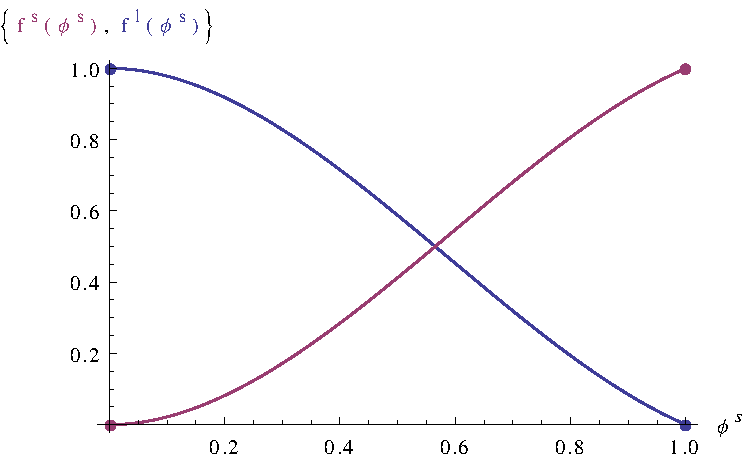
\includegraphics[scale=0.9]{appendix/f_form.pdf}
\caption{A possible form for $f^s$ and  $f^l$.}
\label{}
\end{figure}

Of course the curves for $f^s$ and $f^l$ can be different. We only require that $f^s + f^l = 1$ and that $f^\nu(\phi^s = 0, 1) = \phi^\nu$. 

The simplest form for the curves would be straight lines:
\begin{equation}
	f^\nu = \phi^\nu
\end{equation}
But in that case  using \ref{eq:w} we see that
\begin{equation}
	w^\nu = w
\end{equation}
So if the curves $f^\nu(\phi^s)$ are straight lines, there is no segregation!

We can imagine expanding $f^s$  and $f^l$ in powers of $\phi^s$, $\phi^l$.
\begin{equation} \label{eq:expansion}
	f^\nu = \underbrace{ \phi^\nu }_{\text{order 1}} + \underbrace{ A^\nu_1\phi^s \phi^l }_{\text{order 2}} + 
	\underbrace{ A^\nu_{21} \phi^s (\phi^l)^2 + A^\nu_{22} (\phi^s)^2 \phi^l }_{\text{order 3}} + \text{ ... }
\end{equation}
We know that at order 1, there is no segregation effect. So we will expand $f$ up to order 2 in order to model segregation:
\begin{equation}
	f^\nu = \phi^\nu + A^\nu_1\phi^s \phi^l 
\end{equation}
since $f^s + f^l = 1$ we have 
\begin{equation}
	A^s_1 + A^l_1 = 0
\end{equation}
Let $B = -A^s_1$. We have
\begin{align}
f^s(\phi^s) = \phi^s - B \phi^s (1 - \phi^s) \\
f^l(\phi^s) = 1-\phi^s + B \phi^s (1 - \phi^s) 
\end{align}
Using again \ref{eq:w} we obtain the vertical velocities for the small and large particles. They are respectively
\begin{flalign}
	w^s = w  - \frac{Bg\cos \theta}{c} (1-\phi^s) \\
	w^l = w  + \frac{Bg\cos \theta}{c} \phi^s
\end{flalign}
Note that $q = Bg\cos \theta/c$ is the mean segregation velocity. The coefficients $B$ and $c$ are unknown, but $q$ can be measured directly experimentally.

Substituting $w^s$ the mass balance equation for small particles, we obtain the so-called \textit{segregation equation} for small particles:
\begin{equation}
	\partial_t \phi^s + \partial_x u \phi^s + \partial_y v \phi^s + \partial_z w \phi^s - \partial_z q \phi^s(1-\phi^s) = 0
\end{equation}
Of course, we have a similar equation for large particles:
\begin{equation}
	\partial_t \phi^l + \partial_x u \phi^l + \partial_y v \phi^l + \partial_z w \phi^l + \partial_z q \phi^l(1-\phi^l) = 0
\end{equation}
\subsection{Additional remarks}

Note that doing the transformation $B \leftarrow -B$ is equivalent to doing $g \leftarrow -g$, ie inverting the gravity. Moreover doing the transformation $\phi^s \leftarrow \phi^l$ is equivalent to exchanging the role of small and large particles. Also notice that
\begin{equation}
	f^\nu(\phi^l = 1 - \phi^s; -B) = f^\nu( \phi^s; B)
\end{equation}
That means that the "dual" physical system in which the role of large and small particles is exchanged and the gravity inverted behaves exactly as the normal one. Another way to put it is to say that a large particle in a medium of small ones will be subject to the same force as a small particle in a medium of large ones. Only the direction of the force will be changed. It is not clear at all that this symmetry between a system and its dual exists in real life granular media. 

In fact, this symmetry is a special feature on the expansion at order 2 of \ref{eq:expansion}. At order 3, it disappears. Experiments and finite elements simulations have shown that there is a slight violation of the symmetry between a system and its dual. A third order  theoretical model is currently developed to account for this effect and test its implications.
